
\hzsync{theorem}{6}

\section{\trSymplecticEmbedding{}问题}
\label{sec:symplectic-embeddings}

我们考察 $\R^{m}$ 中具有\trSmooth\trBoundary{}的两个\trCompact、\trConnected{}的%
\trDomain{} $D_{1}$ 与 $D_{2}$。若这两个\trDomain{}经由一个%
\textbf{保\trOriented\trDiffeomorphism}（orientation preserving diffeomorphism）%
而彼此\trDiffeomorphism，便可以提出这样的问题：还需对 $D_{1}$ 与 $D_{2}$ 附加些什么条件，%
才存在一个\trVolumePreserving{}的\trDiffeomorphism，也就是说，一个使得 $\det\varphi'(x)=1$%
对 $D_{1}$ 的\trInterior{}中每个 $x$ 都成立的\trDiffeomorphism{} $\varphi:D_{1}\to D_{2}$？显然，
\[
\operatorname{vol}(D_{1})=\operatorname{vol}(D_{2})
\]
是一个必要条件。而结果表明：对于\trVolumePreserving\trDiffeomorphism{}的存在性而言，%
这已经是唯一同时也是充分的条件。这由下述结果即得——它把 1.3 节中的\cref{thm:moser}\footnote{原书印作「Theorem 2 in Section 3」；原书节引用通例均作「Section N.M」形式，此处系漏排章号之省写，实指 1.3 节中的定理 2（莫泽定理），此处径改。——译者注}%
推广到了带\trBoundary{}的\trManifold{}的情形。

\begin{theorem}[\trDacorogna-\trMoser]\label{thm:dacorogna-moser}
设 $D_{1}$ 与 $D_{2}$ 是 $\R^{m}$ 中两个带\trSmooth\trBoundary{}的\trCompact、%
\trConnected{}的\trDomain。设 $\alpha(x)=a(x)\,dx_{1}\wedge\dots\wedge dx_{m}$%
是 $D_{1}$ 上的一个\trSmooth\trVolumeForm，而 $\beta(x)=b(x)\,dx_{1}\wedge\dots\wedge dx_{m}$%
是 $D_{2}$ 上的一个\trSmooth\trVolumeForm，其中 $a>0$，$b>0$。若 $\varphi:D_{1}\to D_{2}$%
是一个保\trOriented{}\trDiffeomorphism，则存在\trDiffeomorphism{} $\psi:D_{1}\to D_{2}$，%
它此外还满足：在 $\partial D_{1}$ 上 $\psi=\varphi$，并且
\[
\det\bigl(\psi'(x)\bigr)\cdot b\bigl(\psi(x)\bigr)\ =\ \lambda a(x),
\]
其中常数 $\lambda$ 由
\[
\int_{D_{2}}b\ =\ \lambda\cdot\int_{D_{1}}a
\]
给出。
\end{theorem}

特别地，若 $\operatorname{vol}D_{1}=\operatorname{vol}D_{2}$，我们便选取 $a=1$ 与 $b=1$，%
于是得到 $\lambda=1$ 与 $\det\psi'(x)=1$，从而 $\psi$ 是\trVolumePreserving{}的。%
我们由此得出结论：总\trVolume{}是\trVolumePreserving\trDiffeomorphism{}的唯一\trInvariant{}量。%
至于带有对\trBoundary{}与\trVolumeForm{}的精确\trRegularity{}条件的\cref{thm:dacorogna-moser}%
的证明，请参见\trDacorogna{}与\trMoser{}[59]。在特殊情形 $\R^{2}$ 中，%
\trVolumeForm{} $dx_{1}\wedge dx_{2}$ 是一个\trSymplecticForm，于是我们看到：%
单凭总面积就足以把彼此\trDiffeomorphism{}的\trSymplecticManifold{}相互区分开。%
在更高维数时，情形则全然不同。

在\trSymplectic{}空间 $(\R^{2n},\omega_{0})$ 中，人们可以把同样的问题就%
\trSymplecticDiffeomorphism{}（而非\trVolumePreserving\trDiffeomorphism）提出来。%
例如，考察 $\R^{2n}$ 的一个把 $D_{1}$ 映满 $D_{2}$ 的\trSymplecticDiffeomorphism{} $\varphi$。%
于是它把 $D_{1}$ 的\trBoundary{} $\partial D_{1}$ 映到 $\partial D_{2}$ 之上。%
因此，这两个\trHypersurface{}的\textbf{\trCharacteristicLineBundle}（canonical line bundle）%
是\trIsomorphic，而相应的\trHamiltonianFlow{}则在相差一个\trReparametrization{}的意义下彼此\trConjugate。%
特别地，相应的诸\trClosedCharacteristic{}的\trAction{}（如果存在的话）必须彼此一致。%
此外，我们还可以把这些\trBoundary{}加厚成一个由\trHypersurface{}组成的单参数族。%
正如我们将在第 4 章中证明的，一个\trHypersurface{}的\trNeighborhood{}的此种\textbf{\trFoliation}（foliation）之诸\trLeaf（leaf），%
承载着大量的\trClosedCharacteristic。因此，人们会预期存在许多\trSymplecticInvariant；%
而且我们看到，从辛的观点出发去区分彼此\trDiffeomorphism{}的\trDomain{}这一问题，%
与\trVolumePreserving{}的情形相比有着颇为不同的性质。于是，我们转向一个看似较简单但相关的问题：%
考察 $\R^{2n}$ 中的两个开\trDomain{} $U$ 与 $V$，并寻找容许一个%
\trSymplecticEmbedding{} $\varphi:U\to V$ 的那些条件。这就是一个%
\textbf{\trEmbedding}（embedding）$\varphi:U\to\R^{2n}$，%
它此外还满足 $\varphi^{*}\omega_{0}=\omega_{0}$ 与 $\varphi(U)\subset V$。

\noindent\begin{minipage}{\linewidth}
\centering
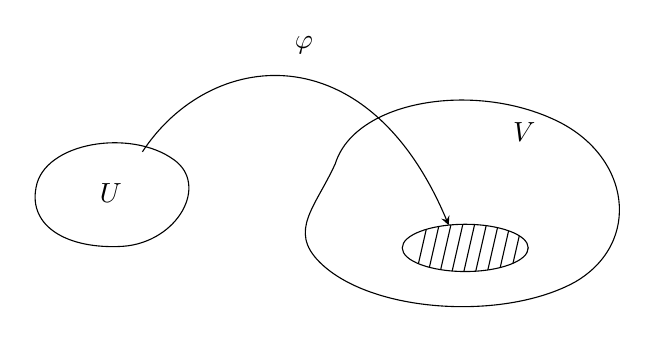
\begin{tikzpicture}[>=stealth]
  \draw (-4.1,0.15) .. controls (-4.0,0.72) and (-2.9,0.9) .. (-2.35,0.5)
        .. controls (-1.9,0.18) and (-2.3,-0.55) .. (-3.0,-0.6)
        .. controls (-3.7,-0.64) and (-4.2,-0.35) .. (-4.1,0.15);%
  \node at (-3.15,0.08) {$U$};
  \draw (-0.3,0.45) .. controls (-0.05,1.25) and (1.45,1.5) .. (2.5,1.0)
        .. controls (3.45,0.55) and (3.6,-0.55) .. (2.75,-1.05)
        .. controls (1.85,-1.55) and (0.15,-1.45) .. (-0.5,-0.8)
        .. controls (-0.9,-0.4) and (-0.55,-0.1) .. (-0.3,0.45);%
  \node at (2.1,0.85) {$V$};
  \begin{scope}%
    \clip (1.35,-0.62) ellipse (0.8 and 0.3);
    \foreach \x in {0.6,0.75,...,2.1}
      \draw (\x,-1.5) -- (\x+0.4,0.25);
  \end{scope}
  \draw (1.35,-0.62) ellipse (0.8 and 0.3);
  \draw[->] (-2.75,0.6) .. controls (-1.9,1.9) and (0.1,2.15) .. (1.14,-0.33);%
  \node at (-0.7,1.95) {$\varphi$};
\end{tikzpicture}

图 1.3
\end{minipage}

由于这样的 $\varphi$ 也是\trVolumePreserving{}的，显然我们有限制条件%
$\operatorname{vol}(U)\leq\operatorname{vol}(V)$。条件 $\operatorname{vol}(U)<\operatorname{vol}(V)$%
对于保证一个\textbf{\trVolumePreserving\trEmbedding}（volume preserving embedding）%
的存在而言已经是充分的。于是问题就产生了：对\trSymplecticEmbedding{}而言，%
除了\trVolume{}之外是否还有其他的\textbf{\trObstruction}（obstruction）？

例如，考察半径 $R>0$ 的一个开\trBall{} $B(R)$：
\[
B(R)=\Bigl\{(x,y)\in\R^{2n}\ \Bigm|\ |x|^{2}+|y|^{2}<R^{2}\Bigr\}
\]
它当然具有有限的\trVolume。它可以很容易地以\trSymplectic{}方式\trEmbedding{}到由
\[
\hat{Z}(r)=\Bigl\{(x,y)\in\R^{2n}\ \Bigm|\ x_{1}^{2}+x_{2}^{2}<r^{2}\Bigr\}
\]
（对每个 $r>0$）所定义的、具有无穷\trVolume{}的那些特殊%
\textbf{开\trCylinder}（cylinder）中去。的确，只需取\trLinear\trSymplecticMapping
\[
\varphi(x,y)=\Bigl(\varepsilon x_{1},\ \varepsilon x_{2},\ x_{3},\ \dots,\ x_{n},\
\frac{1}{\varepsilon}\,y_{1},\ \frac{1}{\varepsilon}\,y_{2},\ y_{3},\ \dots,\ y_{n}\Bigr)
\]
那么，只要把 $\varepsilon>0$ 选得足够小，便有 $\varphi(B(R))\subset\hat{Z}(r)$。%
注意，定义这个\trCylinder{}的 $\R^{2n}$ 中的二维平面 $\operatorname{span}\{e_{1},e_{2}\}$%
是\trIsotropic{}的，从而不承袭任何\trSymplecticStructure。如果我们用\trCylinder
\[
Z(r)=\Bigl\{(x,y)\in\R^{2n}\ \Bigm|\ x_{1}^{2}+y_{1}^{2}<r^{2}\Bigr\}
\]
来取代 $\hat{Z}(r)$，情形就会发生急剧的变化。这个\trCylinder{}由二维平面%
$\operatorname{span}\{e_{1},f_{1}\}$ 所定义，而后者是一个\trSymplectic\trSubspace。%
用\trMapping
\[
\psi(x,y)=\Bigl(\varepsilon x_{1},\ \frac{1}{\varepsilon}\,x_{2},\ x_{3},\ \dots,\ x_{n},\
\varepsilon y_{1},\ \frac{1}{\varepsilon}\,y_{2},\ y_{3},\ \dots,\ y_{n}\Bigr)
\]
作类似的尝试，便可发现当 $\varepsilon$ 小时 $\psi(B(R))\subset Z(r)$。%
\trMapping{} $\psi$ 是\trVolumePreserving{}的。但是，$\psi$ 仅当 $\varepsilon=1$ 时才是\trSymplectic{}的，%
而在这种情形下，也只有当 $r\geq R$ 时才可能有 $\psi(B(R))\subset Z(r)$。%
迄今为止我们都是用\trLinear\trSymplecticMapping{}在做实验，人们或许会指望用%
\trNonlinear\trSymplecticMapping{}做得更好。然而情形并非如此。%
1985 年，M.~\trGromov{}[107] 发现了下述令人惊异的结果。

\begin{theorem}[\trGromov\trSqueezingTheorem]\label{thm:gromov-squeezing}
设在 $B(R)$ 上定义有一个\trSymplecticEmbedding{} $\varphi$，且它满足
\[
\varphi(B(R))\subset Z(r),
\]
则 $r\geq R$（图 1.4）。
\end{theorem}

\noindent\begin{minipage}{\linewidth}
\centering
\begin{tikzpicture}[>=stealth]
  \draw[dashed] (-1.5,3.9) -- (-1.5,3.2);%
  \draw[dashed] (1.5,3.9) -- (1.5,3.2);%
  \draw (-1.5,3.2) -- (-1.5,-0.85);%
  \draw (1.5,3.2) -- (1.5,-0.85);%
  \draw[dashed] (-1.5,-0.85) -- (-1.5,-1.55);%
  \draw[dashed] (1.5,-0.85) -- (1.5,-1.55);%
  \draw (0,1.45) circle (1.26);%
  \draw[dashed] (-1.26,1.45) arc (180:0:1.26 and 0.46);%
  \draw (-1.26,1.45) arc (180:360:1.26 and 0.46);%
  \fill (0,1.45) circle (1.2pt);
  \draw[->] (0,1.45) -- ++(36:1.26);%
  \node at (0.6,1.62) {$R$};
  \draw (-3.8,-0.95) -- (-0.2,-1.62) -- (3.8,-0.72);%
  \draw (-3.8,-0.95) -- (-1.5,-0.43);%
  \draw (1.5,-0.29) -- (3.8,-0.72);%
  \draw[dashed] (-1.5,-0.85) arc (180:0:1.5 and 0.42);%
  \draw (-1.5,-0.85) arc (180:360:1.5 and 0.42);%
  \fill (0,-0.85) circle (1.2pt);
  \draw[->] (0,-0.85) -- (1.5,-0.85);%
  \node at (0.72,-0.62) {$r$};
  \node at (2.55,-0.42) {$(x_{1},y_{1})$-平面};
  \node at (2.45,3.4) {$Z(r)$};
  \draw (1.98,3.12) -- (0.8,3.0);%
\end{tikzpicture}

图 1.4
\end{minipage}

这一现象清楚地表明：一个\trMapping{}的\trSymplecticStructure{}远比\trVolumePreserving{}的结构更具%
\textbf{\trRigidity}（rigidity）。\trGromov{}的这一发现推动了寻求\trSymplecticInvariant{}的工作；%
1987 年，这样的一类\trSymplecticInvariant{}由 I.~\trEkeland{}与 H.~\trHofer{}[68, 69]%
借助一个针对\trHamiltonianEquation{}之\trPeriodicSolution{}的\trVariationalPrinciple{}构造出来；%
这一构造受到了 [67] 中较早结果的启发。这些\trSymplecticInvariant{}将在下一章中予以描述，%
它们将对许多\trSymplecticEmbedding{}的\trRigidity{}现象给出解释，上述结果即属其中。

人们很自然会想从动力学的观点出发，为上述的\trRigidity{}现象给出一个解释。注意，%
\trHypersurface{} $\partial B(R)$ 是\trStandard\trSphere，%
在它上面一切\textbf{\trCharacteristic}（characteristic）都是\trClosed{}的。%
$\partial B(R)$ 是二次\trHamiltonianFunction
\[
H(x,y)=\frac{1}{2}\Bigl(\,|x|^{2}+|y|^{2}\Bigr)
\]
的一个\trEnergySurface。\trHamiltonianEquation{} $\dot{z}=J\nabla H(z)$%
（其中 $z\in\R^{2n}$）是\trLinear{}的，而解
\[
z(t)=e^{Jt}z(0)
\]
满足 $|z(1)|^{2}=|z(0)|^{2}$。它们以 $2\pi$ 为\trPeriodic。此外，%
在 $\partial B(R)$ 上它们全都具有同一个\trAction
\[
A(z)=\pi R^{2},\qquad z(t)\in\partial B(R).
\]
类似地，可以验证：$\partial Z(r)$ 上的\trCharacteristic{}都是\trClosed{}的，绕\trCylinder{}盘旋，%
并且在 $z(t)\subset\partial Z(r)$ 时具有\trAction{} $A(z)=\pi r^{2}$——%
这与 $\partial\hat{Z}(r)$ 上那些为直线的\trCharacteristic{}恰成鲜明对照。%
而如果 $\varphi$ 是 $B(R)$ 的一个\trSymplecticEmbedding，那么在 $\partial\varphi(B(R))$ 上%
\trCharacteristic{}也是\trClosed{}的，并且具有\trAction{} $\pi R^{2}$。%
现在试设想：$B(R)$ 往 $Z(r)$ 之内有一个“最优\trEmbedding”，在此情形下人们倾向于认为，%
被\trEmbedding{}的\trBall{}的\trBoundary{}触到了\trCylinder{}的\trBoundary，%
而且这是沿着一条\trClosedCharacteristic{}发生的。于是，鉴于诸\trAction{}的\trInvariance，%
我们便得出 $r=R$。沿着这些思路的\trGromov{}定理的证明并不存在，%
我们稍后将以不同的方式来进行。
